\documentclass[12pt]{beamer}
\usepackage{graphicx}
\usepackage{fancyvrb}
\fvset{fontsize=\normalsize}
\usepackage{multicol}
\usepackage{booktabs}
\usepackage{units}
\usepackage[T1]{fontenc}
\usepackage{fontspec}
\usepackage[utf8]{inputenc}
\usepackage{helvet}
\usepackage{multicol}
\usepackage{changepage}

\usetheme{default}
\beamertemplatenavigationsymbolsempty
\hypersetup{pdfpagemode=UseNone} 
\setbeameroption{hide notes}
\setbeamertemplate{note page}[plain]

\usetheme{default}
\beamertemplatenavigationsymbolsempty
\hypersetup{pdfpagemode=UseNone} % don't show bookmarks on initial view


\usefonttheme{professionalfonts}
\usefonttheme{serif}
\fontfamily{sans}
\setbeamerfont{note page}{family*=pplx,size=\footnotesize} % Palatin


\definecolor{foreground}{RGB}{255,255,255}
\definecolor{background}{RGB}{24,24,24}
\definecolor{title}{RGB}{107,174,214}
\definecolor{gray}{RGB}{155,155,155}
\definecolor{subtitle}{RGB}{102,255,204}
\definecolor{hilight}{RGB}{102,255,204}
\definecolor{vhilight}{RGB}{255,111,207}
\definecolor{carrotorange}{rgb}{0.93, 0.57, 0.13}

\setbeamercovered{transparent}

\setbeamercolor{titlelike}{fg=title}
\setbeamercolor{subtitle}{fg=subtitle}
\setbeamercolor{institute}{fg=gray}
\setbeamercolor{normal text}{fg=foreground,bg=background}

\setbeamercolor{item}{fg=foreground} % color of bullets
\setbeamercolor{subitem}{fg=gray}
\setbeamercolor{itemize/enumerate subbody}{fg=gray}
\setbeamertemplate{itemize subitem}{{\textendash}}
\setbeamerfont{itemize/enumerate subbody}{size=\footnotesize}
\setbeamerfont{itemize/enumerate subitem}{size=\footnotesize}
\setbeamertemplate{footline}{%
    \raisebox{5pt}{\makebox[\paperwidth]{\hfill\makebox[20pt]{\color{gray}
          \scriptsize\insertframenumber}}}\hspace*{5pt}}

\addtobeamertemplate{note page}{\setlength{\parskip}{12pt}}

\title{Nonparametric covariance estimation for longitudinal data via tensor product smoothing}
\author[The Ohio State University]{Tayler A. Blake}


\setbeamertemplate{footline}{%
    \raisebox{5pt}{\makebox[\paperwidth]{\hfill\makebox[20pt]{\color{gray}
          \scriptsize\insertframenumber}}}\hspace*{5pt}}

% These commands are used to pretty-print LaTeX commands
\newcommand{\bi}{\begin{itemize}}
\newcommand{\ei}{\end{itemize}}
\newcommand{\ig}{\includegraphics}
\newcommand{\subt}[1]{{\footnotesize \color{subtitle} {#1}}}
\newcommand{\newthought}[1]{{\small \color{hilight} {#1}}}
\newcommand{\newmaththought}[1]{{ \color{hilight} {#1}}}
\newcommand{\carrotorangemath}[1]{{ \color{carrotorange} {#1}}}
\newcommand{\ms}{\scriptscriptstyle}

\newcommand{\doccmd}[1]{\texttt{\textbackslash#1}}% command name -- adds backslash automatically
\newcommand{\docopt}[1]{\ensuremath{\langle}\textrm{\textit{#1}}\ensuremath{\rangle}}% optional command argument
\newcommand{\docarg}[1]{\textrm{\textit{#1}}}% (required) command argument
\newenvironment{docspec}{\begin{quote}\noindent}{\end{quote}}% command specification environment
\newcommand{\docenv}[1]{\textsf{#1}}% environment name
\newcommand{\docpkg}[1]{\texttt{#1}}% package name
\newcommand{\doccls}[1]{\texttt{#1}}% document class name
\newcommand{\docclsopt}[1]{\texttt{#1}}% document class option name

\newcommand\myfootnote[1]{%
  \begingroup
  \renewcommand\thefootnote{}\footnote{#1}%
  \addtocounter{footnote}{-1}%
  \endgroup
}





















\begin{document}

%1
{
\setbeamertemplate{footline}{} % no page number here
\frame{
  \titlepage
%  \note{These are slides for a talk I will give on 24 Oct 2013, at a
 %   symposium on open access publishing, organized by the Ebling
   % Library, UW{\textendash}Madison.}
}
}

%2
\begin{frame}
\frametitle{\emph{}}
\newthought{The data:}
\begin{equation*}
Y_i = \left( Y_{i1}, Y_{i2}, \dots, Y_{im} \right)^\prime, \qquad i=1,\dots, N
\end{equation*}
\noindent
associated with measurement times 
\[
t_{1} < t_{2} < \dots< t_{m}.
\]
\end{frame}



%3
%3
%3
\begin{frame}
\frametitle{\emph{The flaming hoops:}}
\bi
\item Covariance matrices (and their estimates) should be positive definite.
	\begin{itemize}
	\item Constrained optimization is a headache.
	\end{itemize} \pause
\item The $\left\{t_{ij} \right\}$ may be suboptimal. 
\begin{itemize}
	\item Observation times may not fall on a regular grid, may vary across subjects.
	\end{itemize} \pause
\item More dimensions, more problems (maybe.)
\begin{itemize}
	\item Sample covariance matrix falls apart when $m$ is large.
	\end{itemize} 
\ei
\end{frame}




%4
%4
%4

\begin{frame}
\frametitle{\emph{The flaming hoops:}}
\bi
\item<4>Covariance matrices (and their estimates) should be positive definite.
	\newthought{A cute little reparameterization } $\color{hilight} \Longrightarrow$ \newthought{unconstrained estimation, meaningful interpretation} 
\item<5> The $\left\{t_{ij} \right\}$ may be messy. \\
	\newthought{Frame covariance estimation as function estimation.} 
\item<6> More dimensions, more problems (maybe.) \\
\begin{figure}
\graphicspath{{img/}}
  
\includegraphics[height=3cm]{ripnatedogg}
  \caption{\color{hilight}\small Regulate like Nate Dogg.}
\end{figure}
\ei
\end{frame}



%5

\begin{frame}
\frametitle{\emph{Covariance dress-up: the modified Cholesky decomposition}}

\begin{equation*}
Y = \left(Y_1, \dots, Y_M \right)^\prime \sim \mathcal{N}\left(0,\Sigma\right).
\end{equation*}

\newthought{For any positive definite} $\color{hilight}{\Sigma}$, \newthought{we can find $T$ which diagonalizes} $\color{hilight}{\Sigma}$:

\begin{equation}
D = T \Sigma T^\prime, \quad T = \begin{bmatrix} 1 & 0 & \dots & & \\ -\phi_{21} & 1 & & & \\ -\phi_{31}& -\phi_{32} &  1 & & \\ \vdots & & & \ddots & \\ -\phi_{M1} &-\phi_{M2} & \dots & -\phi_{M,M-1}& 1  \end{bmatrix}
\end{equation}
\myfootnote{The matrix $T$ is the \emph{Cholesy factor}  of the precision matrix.}
\end{frame}




\begin{frame}
\frametitle{}

\vfill
  \begin{beamercolorbox}[center]{title}
\Large Now, for the cutest part:
  \end{beamercolorbox}
  \vfill

\end{frame}




\begin{frame}
\frametitle{}
\begin{figure}
\graphicspath{{img/}}
  
\includegraphics[height=9cm]{cutest-kitten-ever}
\end{figure}

\end{frame}

%6
\begin{frame}
\frametitle{\emph{Okay, really:}}

Imagine regressing $Y_j$ on its predecessors:

\begin{align} \label{eq:ARmodel}
y_{j}  = \left\{  \begin{array}{ll} 
		e_1 &j=1, \\
  \sum \limits_{k=1}^{j-1} \phi_{jk} y_{k} + \sigma_{j}e_{j} &  j=2,\dots,M
\end{array}\right.
\end{align}
\noindent
In matrix form:
\begin{align}
%\begin{split}
\newmaththought{ e = TY,}
%\end{split}
\end{align}
\noindent
 and taking covariances on both sides:
\begin{equation}
\newmaththought{ D = diag\left( \sigma_1^2,\dots, \sigma_M^2 \right) = T \Sigma T^\prime.}
\end{equation}
\end{frame}








\begin{frame}
\frametitle{\emph{No constraints on the} $\phi_{jk}$s!}

\begin{adjustwidth}{-3cm}{-3cm}
\begin{center}
\begin{figure}
\graphicspath{{img/}}
  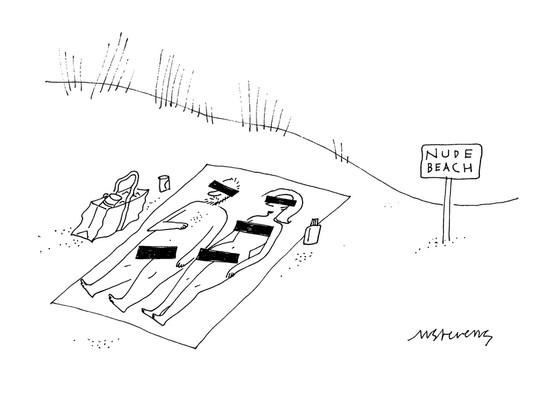
\includegraphics[height=8cm]{nude-beach}
\end{figure}
\end{center}
  \end{adjustwidth}
\end{frame}





\begin{frame}
\frametitle{\emph{The regression model tool box: a deep treasure chest of luxury.}}
Model $Y_j$, $e_j$ as
\begin{align*}
\begin{split}
\newmaththought{Y_j}  \newmaththought{= Y\left( t_j \right) },\quad \newmaththought{e_j}  \newmaththought{= e\left( t_j \right),}\\
\newmaththought{e\left(s\right) \sim  \mathcal{WN}\left(0,1\right),}
\end{split}
\end{align*}
\noindent
Swap the standard regression model \ref{eq:ARmodel} for a varying coefficient model:
\begin{equation*}
\newmaththought{\phi_{jk} = \phi\left(t_j,t_k\right),}
\end{equation*}

\begin{equation}   
\newmaththought{y\left(t_j \right)  = \sum_{k=1}^{j-1} \phi\left(t_j ,t_k\right) y\left(t_k\right) + \sigma\left(t_j\right)e\left({t_j}\right)}
\label{eq:MyModel} 
\end{equation}
\myfootnote{The $\left\{ \phi_{jk} \right\}$ are called \emph{generalized autoregressive parameters}.}
\myfootnote{The $\left\{ \sigma^2_{j} \right\}$ are called the \emph{innovation variances}.}
\end{frame}



\begin{frame}
\frametitle{\emph{(Iterated) penalized maximum likelihood estimation}}

\begin{enumerate}
\item Fix $\sigma_{ij}^2 = \sigma_{ij0}^2$, $i=1,\dots,N$ ,$j=1,\dots,M$.
\item Find $\phi_0 = \underset{\phi}{arg \; min} -2L_\phi\left(\phi, y_1,\dots, y_N \right) + \lambda J\left( \phi \right)$
\item Fix $\phi = \phi_{0}$.
\item Find  $\sigma_{0}^2 = \underset{\sigma^2}{arg\; min} -2L_\sigma^2\left(\sigma^2, y_1,\dots, y_N \right) + \lambda J\left( \sigma^2 \right)$
\end{enumerate}

\begin{adjustwidth}{-2cm}{-2cm}
\begin{equation}
-2 L_\phi\left(\phi, y_1, \dots,y_N \right) = \sum_{i=1}^N \sum_{j=2}^{m_i} \sigma_{ij0}^{-2} \left(y_{ij} - \sum_{k=1}^{j-1}\phi\left({t_{ij},t_{ik}}\right)y_{ik} \right)^2 \label{loglikelihood}
\end{equation}
\end{adjustwidth}
\end{frame}




\begin{frame}
\frametitle{\emph{Regularization of $\phi\left(s,t\right)$ is more intuitive if we transform the $s$-$t$ axis. }}
Rotate the input axes:
\begin{align*}
\newmaththought{l} &\newmaththought{= s-t} \\
\newmaththought{m} &\newmaththought{= \frac{1}{2}\left(s+t\right).}
\end{align*}
\noindent
Then $\phi$ becomes
\begin{align*}
\newmaththought{\phi^*\left(l,m\right)} &\newmaththought{= \phi^*\left(s-t, \frac{1}{2}\left(s+t\right)\right)}\\
 &\newmaththought{= \phi\left(s,t\right).}
\end{align*}

Take $\hat{\phi}^*$ to be the minimizer of 
\[
-2L + \lambda J\left(\phi^*\right)
\]

\end{frame}







\begin{frame}
\frametitle{\emph{Smooth ANOVA models}}
Decompose
\begin{equation} \label{eq:SANOVA-model}
\carrotorangemath{
\phi^*\left(l,m\right) = \mu + \phi_1\left(l\right) + \phi_2\left(m\right) + \phi_{12}\left(l,m\right)},
\end{equation} 
so Model~\ref{eq:MyModel} becomes

\begin{align}  
\begin{split} \label{eq:expanded-ps-anova-vc-model}
\newmaththought{ y\left(t_j \right)  = \sum_{k=1}^{j-1}}\carrotorangemath{ \bigg[\mu + \phi_1\left(l_{jk}\right) + } &\carrotorangemath{\phi_2\left(m_{jk}\right)} \bigg.\\[-2ex]
\bigg. &\carrotorangemath{+ \phi_{12}\left(l_{jk},m_{jk}\right) \bigg]}\newmaththought{y\left(t_k\right)+ \sigma\left(t_j\right)e\left({t_j}\right)}
\end{split}
\end{align}
\end{frame}


\begin{frame}
\frametitle{\emph{We can use B-splines to construct the model basis.}}
Represent the main effects as

\begin{align}  
\begin{split}\label{eq:l-m-marginal-basis}
\newmaththought{\phi_1\left(l\right) } &= \newmaththought{\sum_{c=1}^{c_l} B_{c}\left(l;q_l\right) \theta_{lc }}, \\
\newmaththought{\phi_2\left(m\right) } &= \newmaththought{\sum_{{c^\prime}=1}^{c_m} B_{c^\prime}\left(m;q_m\right)\theta_{mc^\prime } },
\end{split}
\end{align}
and the interaction term by the tensor product of the marginal bases \ref{eq:l-marginal-basis} and \ref{eq:m-marginal-basis}:
\begin{equation} \label{eq:PSANOVA-interaction-term} 
\newmaththought{ \phi_{12}\left(l,m\right)  = \sum_{c=1}^{c_l} \sum_{{c^\prime}=1}^{c_m} B_{c}\left(l;q_l\right) B_{c^\prime  }\left(m;q_m\right)\theta_{c c^\prime } }
\end{equation} 
\end{frame}


\begin{frame}
\frametitle{\emph{PS-ANOVA model basis}}

In matrix notation, Model \ref{eq:expanded-ps-anova-vc-model} becomes

\begin{equation*}  
E \left[ Y | W \right] = WB \theta,
\end{equation*}
\noindent
where $W$ is the matrix of covariates holding the past values of $Y$, and $B$ is the $B$-spline regression basis:
\begin{equation} \label{eq:SANOVA-basis-matrix}
B = \left[\; 1_p \; \vert \;  B_l  \; \vert \;   B_m \; \vert B_{lm} \; \right]
\end{equation}
\noindent
where 
\begin{align*} \label{eq:rowwise-kronecker-product}
B_{lm} &= B_m \; \square \; B_l \\
&\equiv \left( B_m \otimes 1^\prime_{c_l} \right) \odot \left(1^\prime_{c_m} \otimes  B_l  \right).
\end{align*}
\end{frame}





\begin{frame}
\frametitle{\emph{Decomposition of} $\phi^*$ \emph{for} $d_l = d_m = 2$}

%This slide will decompose the function into its parametric and nonparametric components [add a (d_l + 1) x (d_m + 1) two way table with the decompositions of the marginal bases across the margins ]

\begin{table}[h]
%\caption{Decomposition of \phi^* for $d_l = d_m = 2$} %title of the table
\centering % centering table
\begin{tabular}{c|ccccc}
	&    $\left\{ 1 \right\}$	&&	$\left\{m \right\}$	 	&& 	$\left\{ B_{\ms{j^\prime}}\left(m\right) \right\} $ \\ [0.5ex]
\hline % inserts single-line
\\
$\left\{ 1 \right\}$ 				&  $\left\{ 1 \right\}$   	& &	$\left\{m \right\}$	 	&& 	$\left\{ B_{\ms{j^\prime}}\left(m\right) \right\} $	\\  [2.5ex] % Entering row contents
$\left\{l \right\}$		 		&  $\left\{ l \right\}$  	 &&	$l \times m$	 	&& 	$l \times \left\{   B_{\ms{j^\prime}}\left(m\right) \right\} $\\  [2.5ex]
$\left\{ B_j\left(l\right) \right\} $	 	&    $\left\{ B_j\left(l\right) \right\}$	&&	$ m \times \left\{ B_j\left(l\right) \right\}$	& &	$\left\{ B_j\left(l\right) B_{\ms{j^\prime}}\left(m\right) \right\}$ 
\end{tabular}
\end{table}

\end{frame}



\begin{frame}
\frametitle{\emph{Nested PS-ANOVA}}

Re-express $\phi_{\ms{12}}$:

\begin{align*}
\newmaththought{ \phi_{\ms{12}}\left(l,m\right)  =} \carrotorangemath{\; g_{\ms 1}\left(l\right) \Big[ \sum_{r=1}^{\ms{d_m-1}} m^{\ms r}\Big] + \Big[ \sum_{r=1}^{\ms{d_l-1}} l^{\ms r} \Big] g_{\ms 2}\left(m\right)\;}  \newmaththought{+ h\left( l,m \right), } 
\end{align*}
\noindent
For $d_l = d_m = 2$,
\[
\newmaththought{ \phi_{\ms{12}}\left(l,m\right)  =} \carrotorangemath{\; g_{\ms 1}\left(l\right) \; m+ l \; g_{\ms 2}\left(m\right)\;}\newmaththought{ + \; h\left( l,m \right) } 
\]
with basis:
\begin{equation} \label{eq:nested-SANOVA-basis-matrix}
\color{hilight}{B = \big[ } \; 1_p \; \vert \;  B_1  \; \vert \;   B_2 \; \vert \carrotorangemath{ B_3 \; \vert B_4 }\;\newmaththought{ \vert B_5 \; \big]},
\end{equation}
\noindent
where
\begin{align*}
\carrotorangemath{B_{\ms 3}\;} &\carrotorangemath{= \;m \;} \carrotorangemath{ \square \;  B_{\ms 1}}  &  \newmaththought{B_{\ms 5}\;}\newmaththought{=\; B_{\ms 2} \;} \newmaththought{ \square \; B_{\ms 1} } \\
 \carrotorangemath{B_{\ms 4}\;}&\carrotorangemath{=\; B_{\ms 2} \;} \carrotorangemath{ \square \; l } &
\end{align*}


\end{frame}




\begin{frame}
\frametitle{\emph{Nested PS-ANOVA}}



\end{frame}



































\end{document}